% #############################################################################
% This is Chapter 5
% !TEX root = ../main.tex
% #############################################################################
% Change the Name of the Chapter i the following line
\fancychapter{Fatori-V with IOb-SoC-Ibex}
% The following line allows to ref this chapter
\label{chap5:ibex}

% #############################################################################
\section{Ibex Overview}
\label{chap5:ibex_overview}

Ibex \cite{ibex} is the open-source \ac{RISC-V} core, developed by lowRISC, selected as the \ac{Fatori-V} baseline. \Cref{fig:ibex} shows its pipeline and its integration with IOb-SoC.

\begin{figure}[h]
    \centering
    \begin{subfigure}{0.4\textwidth}
        \centering
        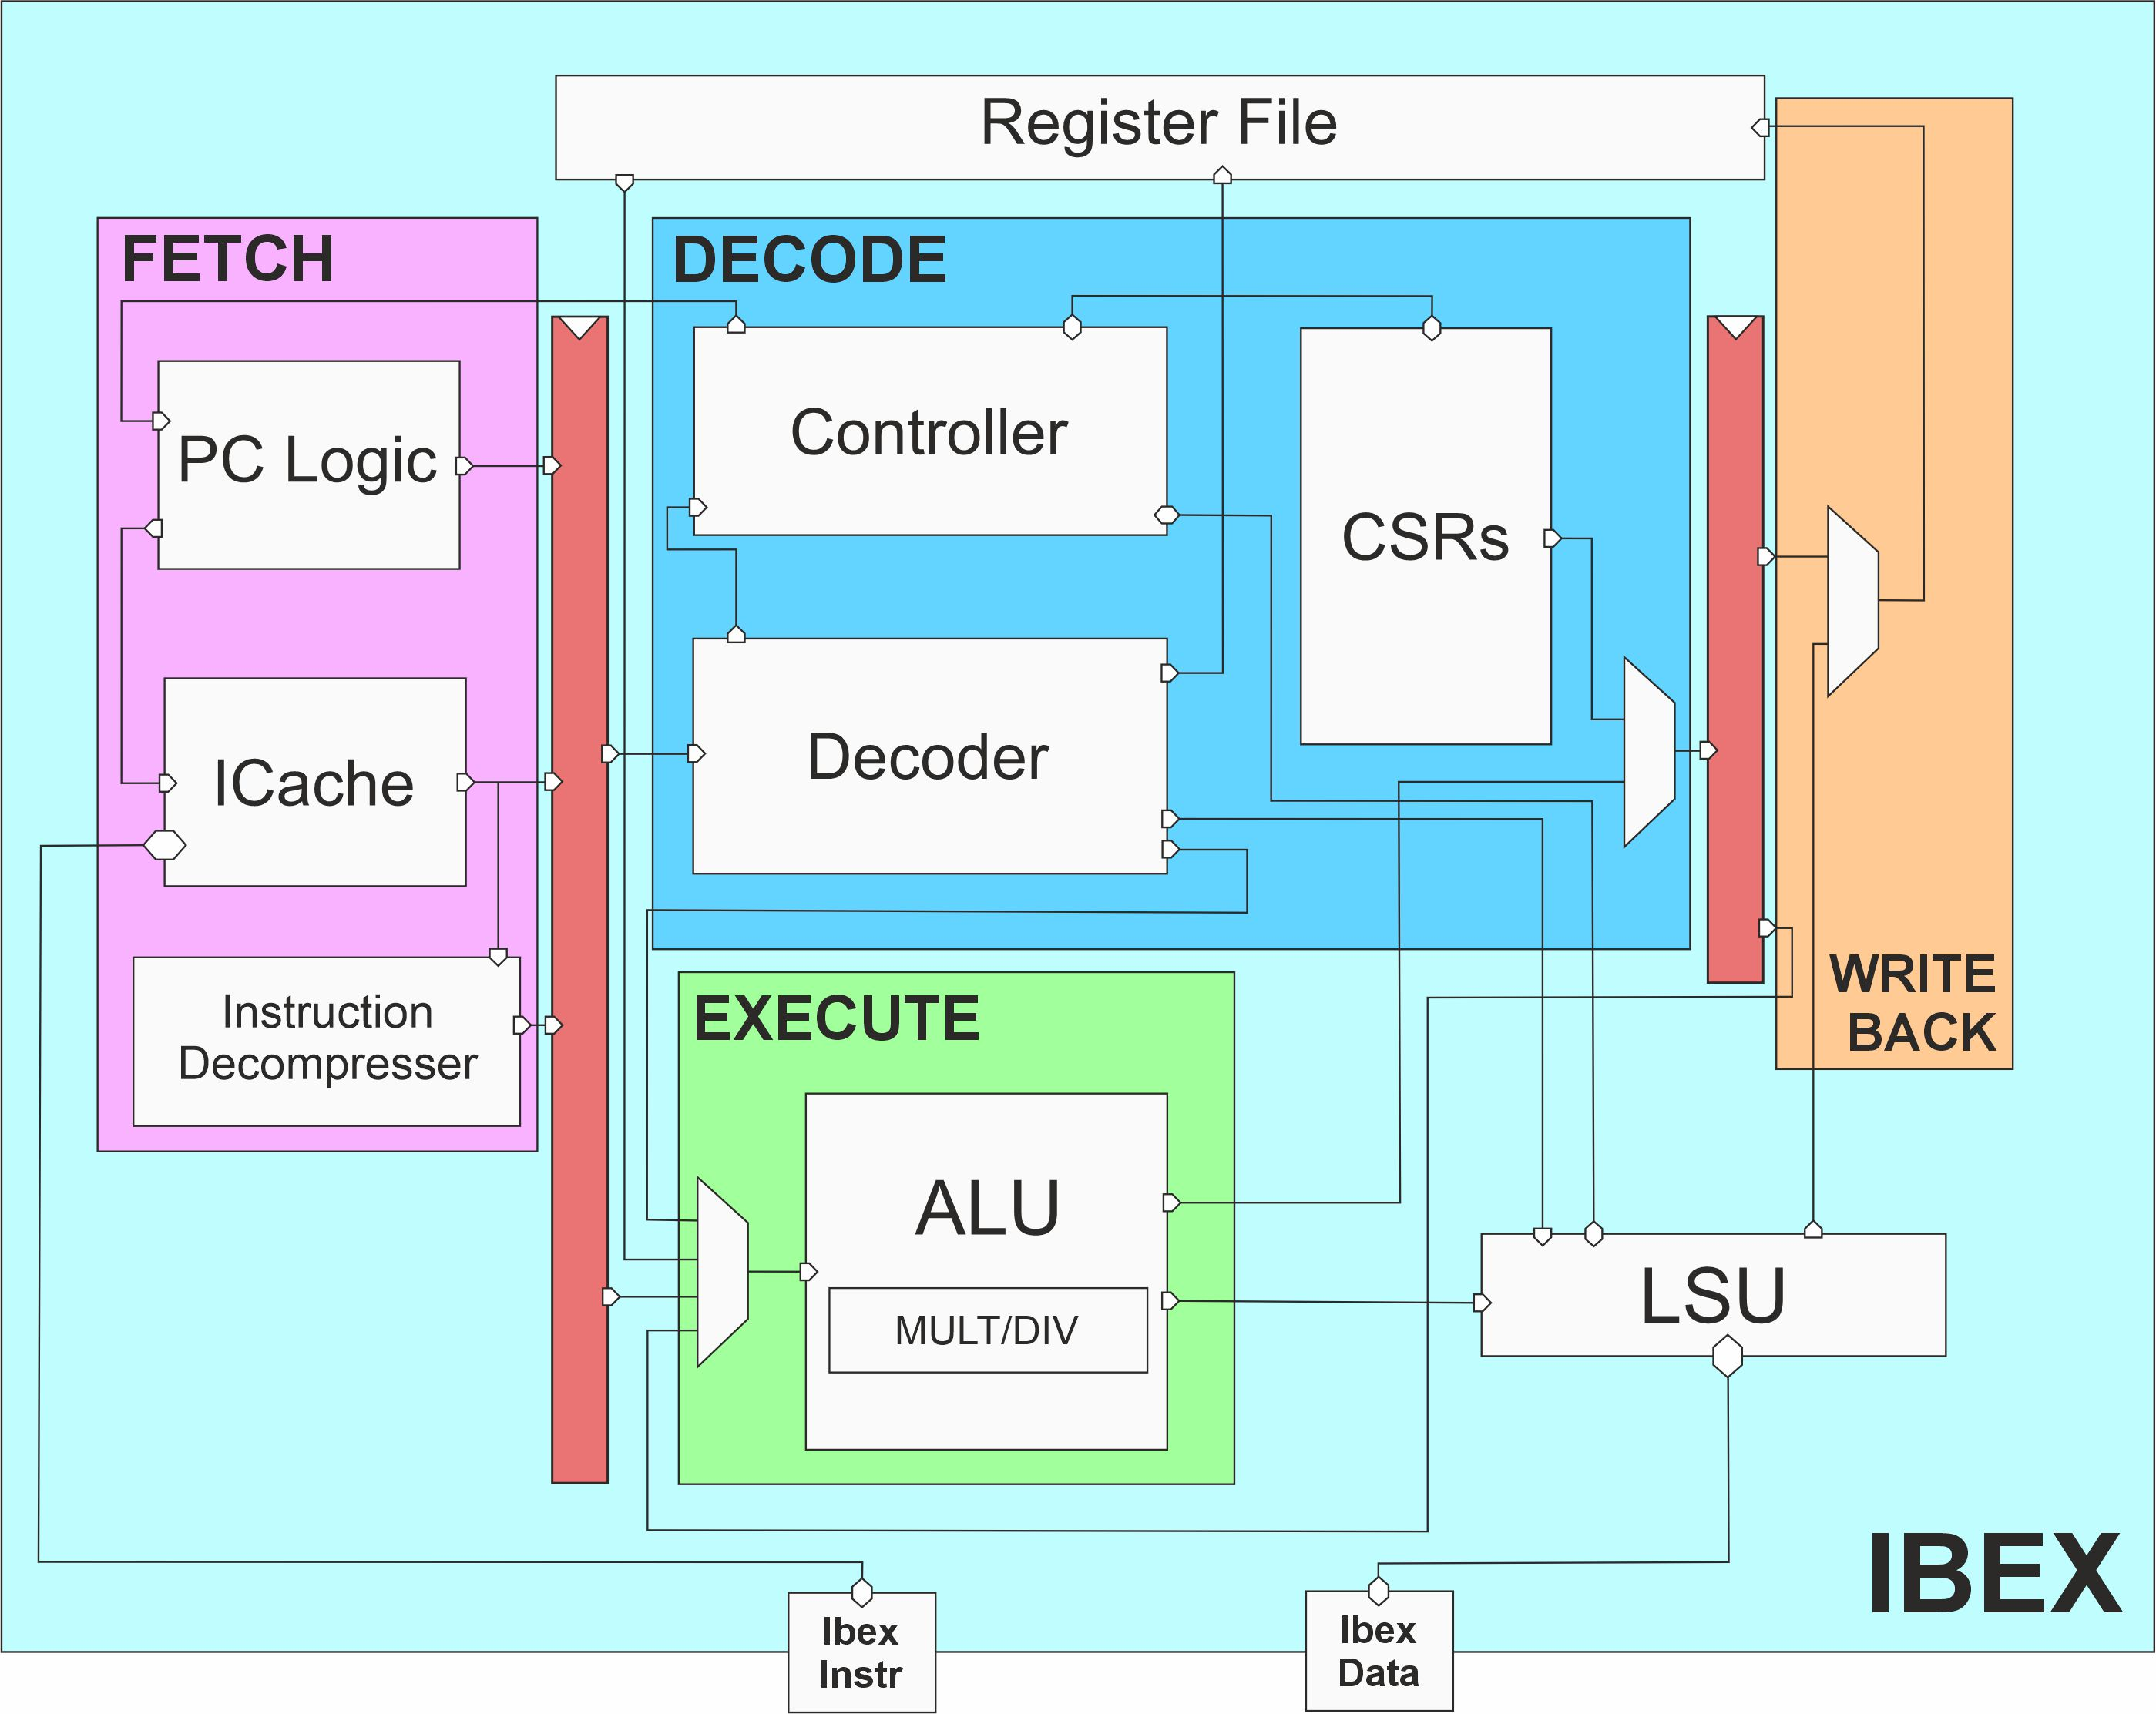
\includegraphics[width=\linewidth]{Images/chap5_ibex.jpg}
        \caption{Ibex Core}
        \label{fig:ibex_cpu}
    \end{subfigure}
    \hfill
    \begin{subfigure}{0.55\textwidth}
        \centering
        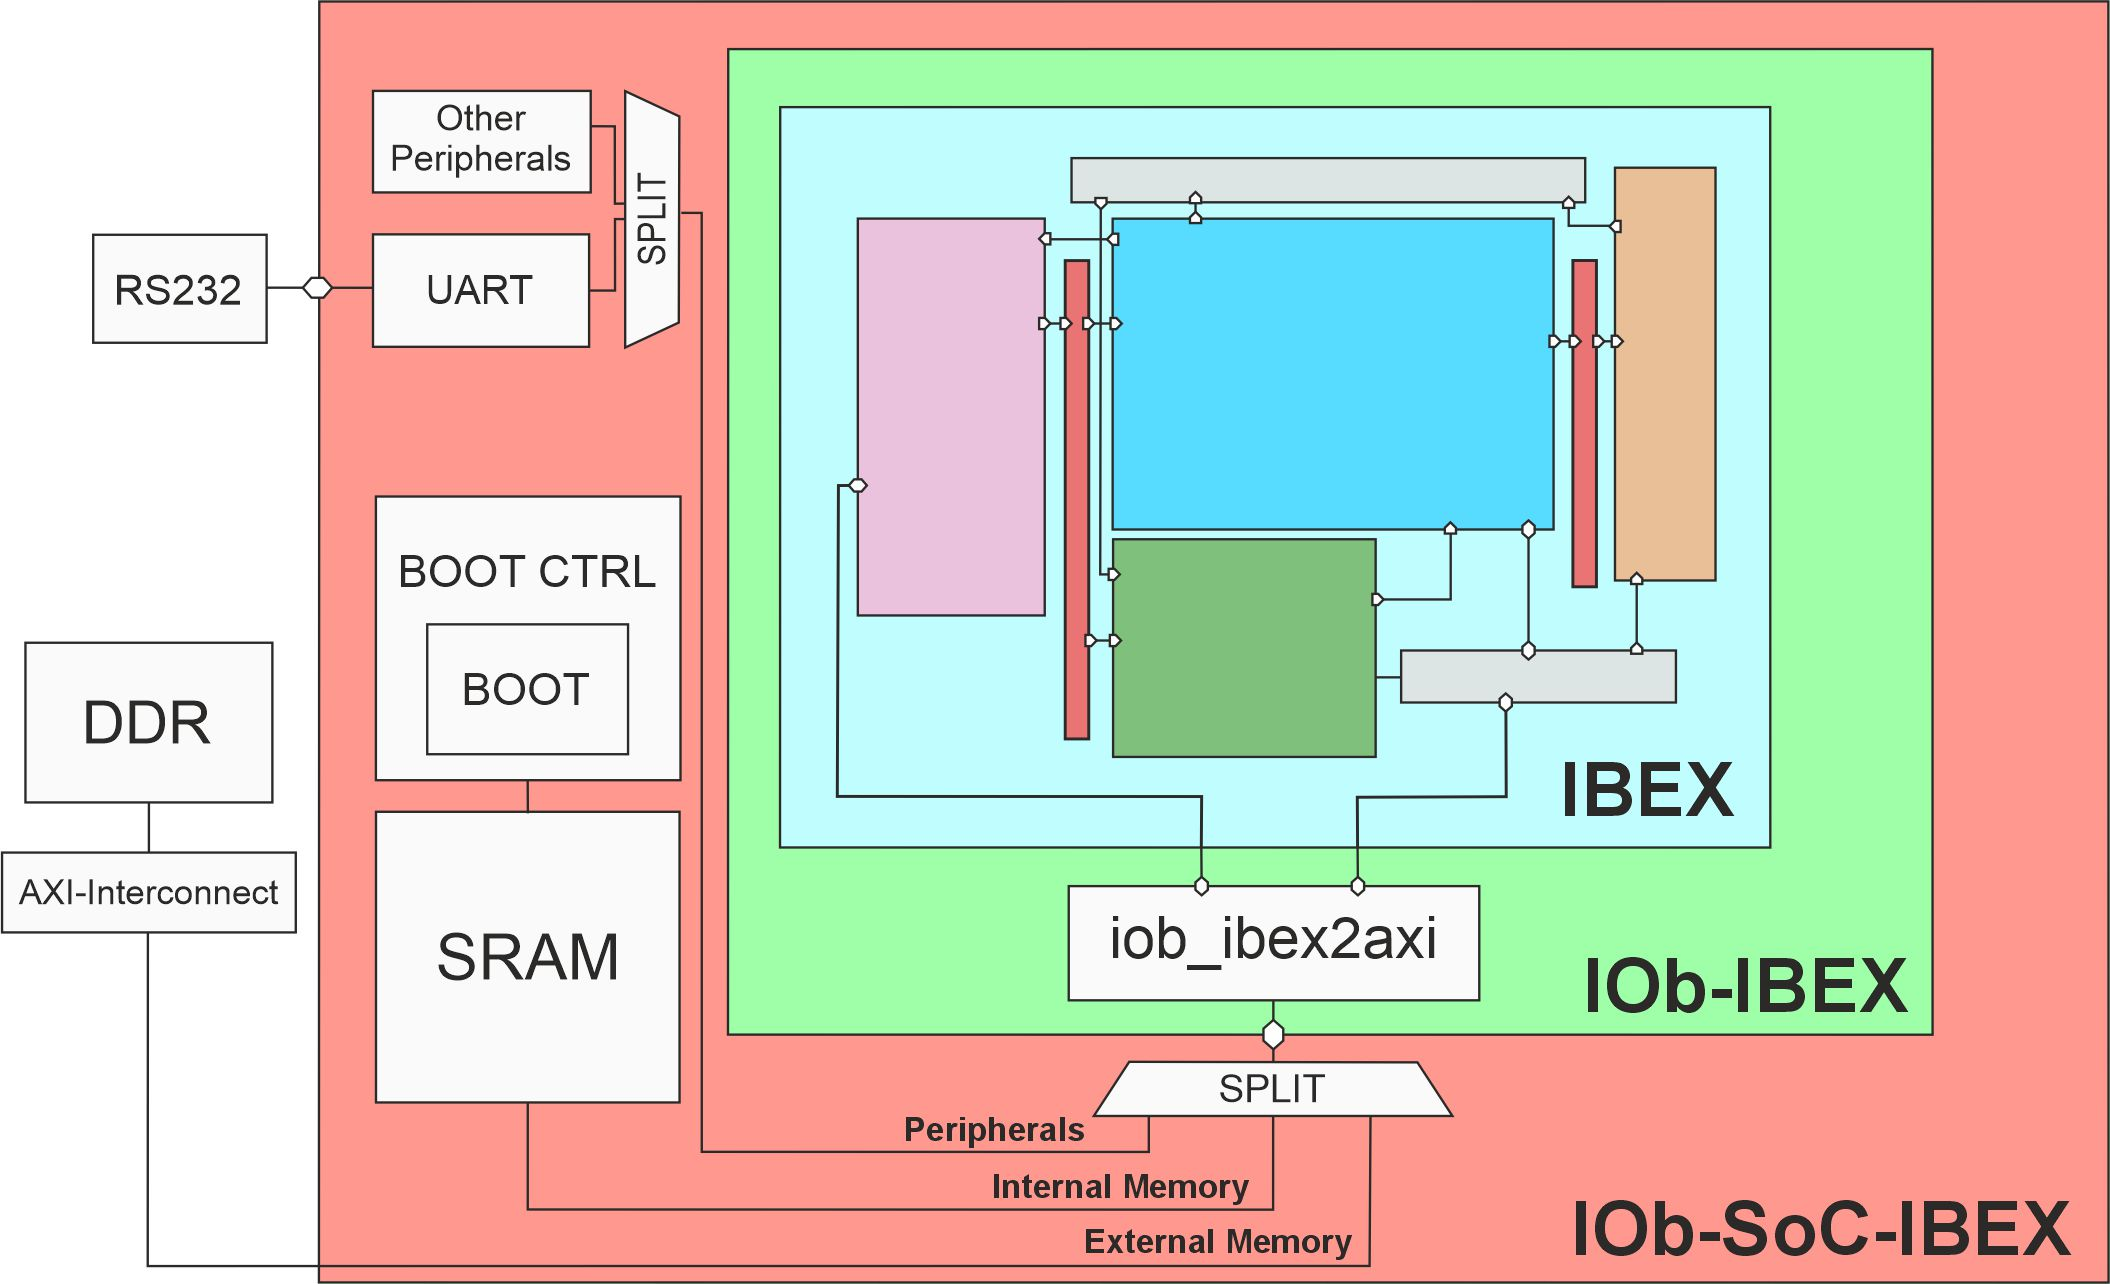
\includegraphics[width=\linewidth]{Images/chap5_iob-soc-ibex.jpg}
        \caption{Ibex + IOb-SoC Integration}
        \label{fig:ibex+iob}
    \end{subfigure}
    \caption{Ibex Overview}
    \label{fig:ibex}
\end{figure}

Ibex is a 32-bit in-order \ac{RISC-V} core used across the lowRISC ecosystem, most notably in OpenTitan. It uses a 2-stage baseline pipeline with an optional writeback stage and exposes separate instruction and data memory ports through a request/grant/response handshake. Ibex supports RV32I or RV32E with the C, M, and B extensions, and offers microarchitectural options affecting area, performance, and \ac{FT}, including register-file implementation, branch optimizations, and a choice between prefetch buffer and instruction cache.

Ibex implements the standard \ac{RISC-V} \ac{CSR} set. The counters used for performance monitoring in this work are listed in \Cref{tab:ibex_perf_csrs_example}.

\begin{table}[h]
\centering
\begin{tabularx}{\textwidth}{|l|l|l|X|}
\hline
\rowcolor{tableheader}\textbf{Address} & \textbf{Name} & \textbf{\ac{Fatori-V} Alias} & \textbf{Description}\\
\hline
\hline
\texttt{0xB00} & \texttt{mcycle} & \texttt{mcycle} & Total cycles; upper 32 bits at \texttt{0xB80}\\
\hline
\texttt{0xB02} & \texttt{minstret} & \texttt{minstret} & Retired instructions; upper 32 bits at \texttt{0xB82}\\
\hline
\texttt{0xB03} & \texttt{mhpmcounter3} & \texttt{hpm\_lsu\_busy} & Cycles waiting for data memory (\texttt{NumCyclesLSU})\\
\hline
\texttt{0xB04} & \texttt{mhpmcounter4} & \texttt{hpm\_ifetch\_stall} & Cycles waiting for instruction fetch (\texttt{NumCyclesIF})\\
\hline
\texttt{0xB05} & \texttt{mhpmcounter5} & \texttt{hpm\_loads} & Number of loads (\texttt{NumLoads})\\
\hline
\texttt{0xB06} & \texttt{mhpmcounter6} & \texttt{hpm\_stores} & Number of stores (\texttt{NumStores})\\
\hline
\texttt{0xB07} & \texttt{mhpmcounter7} & \texttt{hpm\_jumps} & Number of jumps (\texttt{NumJumps})\\
\hline
\texttt{0xB08} & \texttt{mhpmcounter8} & \texttt{hpm\_branches} & Number of branches (\texttt{NumBranches})\\
\hline
\texttt{0xB09} & \texttt{mhpmcounter9} & \texttt{hpm\_branches\_taken} & Taken branches (\texttt{NumBranchesTaken})\\
\hline
\texttt{0xB0A} & \texttt{mhpmcounter10} & \texttt{hpm\_compressed} & Compressed instructions retired (\texttt{NumInstrRetC})\\
\hline
\texttt{0xB0B} & \texttt{mhpmcounter11} & \texttt{hpm\_multiply\_stalls} & Cycles waiting for multiply (\texttt{NumCyclesMulWait})\\
\hline
\texttt{0xB0C} & \texttt{mhpmcounter12} & \texttt{hpm\_divide\_stalls} & Cycles waiting for divide (\texttt{NumCyclesDivWait})\\
\hline
\end{tabularx}
\caption{Ibex \acp{CSR} used as counters. All entries are R/W in M-mode; writes are used only to reset counters to zero.}
\label{tab:ibex_perf_csrs_example}
\end{table}





% #############################################################################
\section{Ibex and Fault Tolerance}
\label{chap5:ibex_ft}

Ibex was selected partly because it includes native \ac{FT}-related support. This section reviews the native Ibex \acp{FTM} and details the native \ac{FT} features relevant to \ac{Fatori-V}'s development.

Ibex's native \ac{FT} mechanisms, introduced in \Cref{chap2:ftms}, are enabled through the SecureIbex configuration. These include Dual-Core Lockstep, Shadow \acp{CSR}, register-file and ICache \ac{ECC}, bus integrity checking, a hardened \ac{PC}, and several control-signal glitch protections. Data Independent Timing and Dummy Instructions are also available, but target side-channel and fault-injection attack resistance rather than \ac{SEU} mitigation.

Ibex does not provide complete error handling hardware by default, but it exposes control and status ports that can be used by integration logic to detect faults and trigger recovery. These ports, listed in \Cref{tab:ibex_error_ports}, include three alert outputs, a multi-bit fetch-enable input that can stop instruction fetching, a sleep indicator that reports core activity, and a double-fault flag.

However, Ibex only exposes these ports. It does not aggregate errors across the \ac{SoC}, count error occurrences, or compute any \ac{FT}-related metrics. Furthermore, alert outputs are status signals, not counters, meaning that they remain asserted until cleared. Counting detections, extracting quantitative \ac{FT} metrics, and reacting to reported errors requires the implementation of a fault manager.

\begin{table}[h]
\centering
\begin{tabularx}{\textwidth}{|l|l|c|X|}
\hline
\rowcolor{tableheader}\textbf{Signal} & \textbf{Direction} & \textbf{Width} & \textbf{Description} \\
\hline
\hline
alert\_minor\_o &
Output & 1 &
Reports recoverable events that do not require external intervention (e.g.\ corrected \ac{ECC}, retryable check). \\
\hline
alert\_major\_internal\_o &
Output & 1 &
Reports a non-recoverable condition detected inside the core (e.g.\ lockstep mismatch, \ac{PC} progression fault, \ac{CSR} shadow mismatch). \\
\hline
alert\_major\_bus\_o &
Output & 1 &
Reports a non-recoverable condition detected on incoming bus data (e.g.\ bad checkbits, corrupted load or instruction data). \\
\hline
double\_fault\_seen\_o &
Output & 1 &
Indicates a second fault was detected before the first was cleared (e.g.\ major alert raised while a previous major is still set). \\
\hline
fetch\_enable\_i &
Input & 4 &
Multi-bit input that controls whether the core fetches instructions. \\
\hline
core\_sleep\_o &
Output & 1 &
Goes high when the core has flushed with no outstanding transactions. \\
\hline
\end{tabularx}
\caption{Ibex error control ports}
\label{tab:ibex_error_ports}
\end{table}




% #############################################################################
\section{System-on-Chip Integration}
\label{chap5:soc-integration}

IOb-\ac{SoC}-Ibex is a \ac{SoC} built on IOb-\ac{SoC} with Ibex as the \ac{CPU}, developed using the Py2HWSW Python framework for hardware generation and building. The framework and the integration process are detailed in \Cref{chap5:py2hwsw,chap5:iob-soc-ibex}.





% -------------------------------------------------------------
\subsection{Py2HWSW Infrastructure}
\label{chap5:py2hwsw}

Py2HWSW is a Python-based framework for embedded hardware and software design. A system is described through \texttt{.py} entry files that declare modules, connections, and parameters; the framework then generates a complete project workspace with \ac{RTL}, software support, and build infrastructure for simulation, synthesis, and \ac{FPGA} bitstream generation. It separates user sources (Setup Directory), framework library (Py2HWSW Directory), and generated output (Build Directory, which can be deleted and regenerated). IOb-\ac{SoC} and IOb-\ac{SoC}-Ibex are both Setup Directories built with this model.



% -------------------------------------------------------------
\subsection{IOb-SoC-Ibex}
\label{chap5:iob-soc-ibex}

The top layer, IOb-SoC-Ibex, is forked from IOb-SoC with Ibex selected as the \ac{CPU}. Two hook mechanisms were added to make it externally configurable: a Vivado \ac{TCL} hook that sources user-provided scripts at fixed synthesis stages, and a benchmark hook that compiles sources from an external directory instead of the default firmware. Since Ibex relies on SystemVerilog packages, the \ac{FPGA} build flow was also modified to compile SystemVerilog package files before other sources, as shown in \Cref{lst:src_order}.

\begin{lstlisting}[float=h,language=matlabfloz,caption={Portion of the modified Py2HWSW \ac{FPGA} Makefile enforcing package ordering}, label={lst:src_order}]
VHDR+=$(wildcard ../src/*.vh) $(wildcard ./src/*.vh)
PCKS+=$(wildcard ../src/*_pkg.sv)
VSRC+=$(PCKS)
SVRC+=$(wildcard ../src/*.sv)
VSRC+=$(filter-out $(PCKS), $(SVRC))
VSRC+=$(wildcard ../src/*.v) $(wildcard ./src/*.v)
\end{lstlisting}

IOb-Ibex, the second layer, wraps the Ibex \ac{RTL} for the Py2HWSW build tree. Only locally modified files are stored in \texttt{hardware/src/}; the remaining Ibex sources are generated from the official repository and copied into the Build Directory by dedicated Makefile targets, so that local fixes take priority. Since Ibex is SystemVerilog-based, automatic \ac{HDL} generation is disabled and the wrapper is provided manually as \texttt{iob\_ibex.sv}.

The third layer is the official Ibex repository, included as a submodule of IOb-Ibex; its FuseSoC export flow is invoked through the Ibex-Demo-System \cite{ibex-demo-system} Nix environment to produce the full set of SystemVerilog sources.





% -------------------------------------------------------------
\subsection{AXI Bridge for Ibex}
\label{chap5:ibex2iob}

IOb-SoC connects the \ac{CPU} to memory and peripherals through an \ac{AXI} bus, while Ibex uses a simpler request, grant, and response handshake on separate instruction and data ports. To bridge these interfaces, a dedicated AXI-to-Ibex hardware bridge was developed and instantiated in the \ac{CPU} wrapper. \Cref{fig:ibex_protocol} illustrates the native Ibex LSU protocol, where a request stays asserted until granted, and completion is signalled by a one-cycle response pulse that may include data and an error flag.

\begin{figure}[h]
\centering
    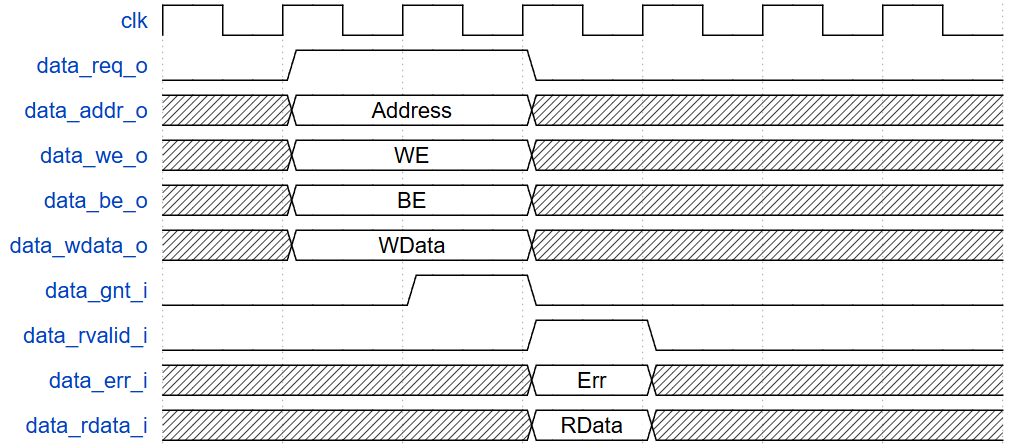
\includegraphics[width=0.9\textwidth]{./Images/Ibex Protocol.png}
    \caption{Ibex LSU interface timing diagram. Ibex' perspective.}
    \label{fig:ibex_protocol}
\end{figure}

The developed module, \texttt{iob\_ibex2axi} shown in \Cref{fig:ibex+iob}, provides Ibex-facing ports on one side and an \ac{AXI} interface toward IOb-SoC on the other. In this version, the adapter targets the subset of signals needed for a functioning \ac{SoC} integration, translating the core read and write transactions into an \ac{AXI}-Lite style behaviour. Advanced \ac{AXI} features such as burst transfers are not implemented, and unused attributes are tied to default values. The Ibex core ports connected by the adapter are listed in \Cref{tab:ibex2axi_ibex} and the \ac{AXI}-side ports of the wrapper in \Cref{tab:ibex2axi_axi}.

On a memory request, Ibex raises the request signal alongside the address and, for stores, the write-enable, byte-enables, and write data. The bridge maps these to the corresponding \ac{AXI} address and data channels, asserts the grant once the slave is ready, and returns a one-cycle completion pulse with read data or an error flag.

\begin{table}[h]
\centering
\small
\setlength{\tabcolsep}{3.2pt}
\renewcommand{\arraystretch}{1.25}
\begin{tabularx}{\textwidth}{|l|l|c|X|}
\hline
\rowcolor{tableheader}\textbf{Name} &
\textbf{Direction} &
\textbf{Width} &
\textbf{Description} \\
\hline
\hline
\texttt{ibex\_instr\_req\_i}, \texttt{ibex\_data\_req\_i} &
Input & 1 &
Memory access request, held by Ibex until accepted by the adapter. \\
\hline
\texttt{ibex\_instr\_addr\_i}, \texttt{ibex\_data\_addr\_i} &
Input & 32 &
Target address for instruction fetch, load, or store. \\
\hline
\texttt{ibex\_data\_we\_i} &
Input & 1 &
Selects store access (high) or load access (low). \\
\hline
\texttt{ibex\_data\_be\_i} &
Input & 4 &
Byte enables for store accesses. \\
\hline
\texttt{ibex\_data\_wdata\_i} &
Input & 32 &
Write data for store accesses. \\
\hline
\texttt{ibex\_instr\_gnt\_o}, \texttt{ibex\_data\_gnt\_o} &
Output & 1 &
Signals that the adapter accepted the Ibex request. \\
\hline
\texttt{ibex\_instr\_rvalid\_o}, \texttt{ibex\_data\_rvalid\_o} &
Output & 1 &
One-cycle completion pulse for read and write accesses. \\
\hline
\texttt{ibex\_instr\_rdata\_o}, \texttt{ibex\_data\_rdata\_o} &
Output & 32 &
Read data returned to the core. \\
\hline
\texttt{ibex\_instr\_err\_o}, \texttt{ibex\_data\_err\_o} &
Output & 1 &
Signals an error when the completed \ac{AXI} transaction reports an error response. \\
\hline
\end{tabularx}
\caption{Ibex core ports connected by \texttt{iob\_ibex2axi}.}
\label{tab:ibex2axi_ibex}
\end{table}

\begin{table}[h]
\centering
\small
\setlength{\tabcolsep}{3.2pt}
\renewcommand{\arraystretch}{1.25}
\begin{tabularx}{\textwidth}{|l|l|c|X|}
\hline
\rowcolor{tableheader}\textbf{Name} &
\textbf{Direction} &
\textbf{Width} &
\textbf{Description} \\
\hline
\hline
\texttt{ibus\_arvalid\_o}, \texttt{dbus\_arvalid\_o} &
Output & 1 &
Read address valid; used for instruction fetches and loads. \\
\hline
\texttt{ibus\_araddr\_o}, \texttt{dbus\_araddr\_o} &
Output & 32 &
Read address for instruction fetches and loads. \\
\hline
\texttt{dbus\_awvalid\_o} &
Output & 1 &
Write address valid; used for stores. \\
\hline
\texttt{dbus\_awaddr\_o} &
Output & 32 &
Write address for stores. \\
\hline
\texttt{dbus\_wvalid\_o} &
Output & 1 &
Write data valid; used for stores. \\
\hline
\texttt{dbus\_wdata\_o} &
Output & 32 &
Write data for stores. \\
\hline
\texttt{dbus\_wstrb\_o} &
Output & 4 &
Write byte strobes for stores. \\
\hline
\texttt{ibus\_rready\_o}, \texttt{dbus\_rready\_o}, \texttt{dbus\_bready\_o} &
Output & 1 &
Read-data and write-response ready signals; hardwired to~1. \\
\hline
\texttt{ibus\_arready\_i}, \texttt{dbus\_arready\_i} &
Input & 1 &
Indicates that the \ac{AXI} slave accepted the read address. \\
\hline
\texttt{ibus\_rvalid\_i}, \texttt{dbus\_rvalid\_i} &
Input & 1 &
Read data valid from the \ac{AXI} slave. \\
\hline
\texttt{ibus\_rdata\_i}, \texttt{dbus\_rdata\_i} &
Input & 32 &
Read data returned by the \ac{AXI} slave. \\
\hline
\texttt{ibus\_rresp\_i}, \texttt{dbus\_rresp\_i} &
Input & 2 &
Read response status returned by the \ac{AXI} slave. \\
\hline
\texttt{dbus\_wready\_i} &
Input & 1 &
Indicates that the \ac{AXI} slave accepted the write data. \\
\hline
\texttt{dbus\_bvalid\_i} &
Input & 1 &
Write response valid from the \ac{AXI} slave. \\
\hline
\texttt{dbus\_bresp\_i} &
Input & 2 &
Write response status returned by the \ac{AXI} slave. \\
\hline
\end{tabularx}
\caption{\texttt{iob\_ibex2axi} wrapper \ac{AXI} interface ports.}
\label{tab:ibex2axi_axi}
\end{table}

The bridge is implemented through direct combinational assignments. Load and store requests are distinguished by \texttt{ibex\_data\_we\_i}: reads drive the \ac{AXI} read-address channel ($\texttt{dbus\_arvalid\_o} = \texttt{ibex\_data\_req\_i} \mathbin{\&} \sim\texttt{ibex\_data\_we\_i}$) while stores drive the write-address and write-data channels ($\texttt{dbus\_awvalid\_o} = \texttt{dbus\_wvalid\_o} = \texttt{ibex\_data\_req\_i} \mathbin{\&} \texttt{ibex\_data\_we\_i}$). The completion signal merges read and write responses into the single indication Ibex expects: $\texttt{ibex\_data\_rvalid\_o} = \texttt{dbus\_rvalid\_i} \mathbin{||} \texttt{dbus\_bvalid\_i}$. Unused \ac{AXI} fields are tied to default values, limiting the bridge to single transfers.


% #############################################################################
\section{Summary}
\label{chap5:summary}

This chapter presented the IOb-SoC-Ibex baseline. The Ibex core was introduced, covering its pipeline, configuration options, \ac{CSR}-based performance monitoring interface, and native \ac{FT} mechanisms. The integration work that produced IOb-SoC-Ibex was then described: the Py2HWSW build infrastructure and its three-directory model, the three-layer repository structure that separates the \ac{SoC} project, the Ibex wrapper, and the official Ibex sources, and the \ac{AXI} bridge developed to connect the Ibex memory handshake to the IOb-SoC bus. \Cref{chap6:fatori_hardware} details the \ac{FTM} hardware and fault manager built on top of this baseline.





